% !TeX root = ../bbchallenge-paper.tex

\newcommand{\ngramcps}{NGramCPS\xspace}

\subsection{$n$-gram Closed Position Set (\ngramcps)}\label{sec:n-gramCPS}

The $n$-gram Closed Position Set (\ngramcps) decider which we introduce here is a simplification of an earlier technique, Closed Position Set (CPS), itself introduced in \texttt{bbfind} \cite{Skelet_bbfind}, see Section~\ref{sec:intro:mainresults}. Surprisingly, \ngramcps is a relatively simple technique which makes a potent decider as it decides 99.89\% of all nonhalting enumerated 5-state machines excluding loops, see Table~\ref{tab:pipelineBB5}.

The method is especially potent when augmenting the binary alphabet of Turing machines to record extra information on the tape, such as a fixed-length history of previously seen (state,symbol) pairs, see Section~\ref{sec:n-gramCPS:augmentations}.

\subsubsection{\ngramcps algorithm}\label{sec:n-gramCPS:algo}

Algorithm~\ref{alg:NGramCPS} gives a pseudo-code of the \ngramcps decider. The decider considers finite, \textit{local configurations} of a Turing machine consisting of: (i) the \textit{$n$-grams} (see after) respectively to the left and to the right of the head, (ii) the state the machine is in, and (iii) the symbol currently read by the head, referred to as \textit{middle} symbol (as opposed to the left and right part of the tape, modelled by the n-grams). By \textit{$n$-gram}, we mean a sequence of $n > 0$ symbols from the tape alphabet (for instance, the binary alphabet $\alphabet=\{\szero,\sone\}$).

The algorithm builds a set of local configurations \textit{potentially} reachable by the machine until either an undefined transition is met (Algorithm~\ref{alg:NGramCPS}, l.\ref{alg:NGramCPS:line:unknown}) or no new configurations are added to the set, i.e. the set is closed under Turing machine operations (Algorithm~\ref{alg:NGramCPS}, l.\ref{alg:NGramCPS:line:nonhalt}). In the first case, the decider cannot conclude and the machine is left undecided. In the second case, the decider concludes that the machine does not halt as no undefined transition (\ie where the machine could be asked to halt) can be reached.

The central idea of this decider and the reason behind using the ``$n$-gram'' terminology (originating from \textit{$n$-gram models} in language analysis)  is better illustrated by the following example. Let $n=3$ and consider local configuration \texttt{011 [B0] 100}, meaning that the left $n$-gram is \texttt{011}, right $n$-gram is \texttt{100}, the machine is in \stateB and reading symbol \texttt{0}. Assume that the  machine's transition for reading a \texttt{0} in state \stateB is \texttt{1RC}, meaning that the machine writes \texttt{1}, moves right and transitions to state \stateC. The local configuration becomes \texttt{011 1 [C1] 00?}, where \texttt{?} means that we don't know which symbol to use. Then:

\begin{enumerate}
    \item \textbf{Left $n$-gram update.} We record the left $n$-gram \texttt{011} as seen (it is inserted in set $L$, Algorithm~\ref{alg:NGramCPS}, l.\ref{alg:NGramCPS:line:insertL}) and we discard its first bit, updating the left $n$-gram to \texttt{111}. The local configuration becomes \texttt{111 [C1] 00?}.
    \item \textbf{Right $n$-gram update.} In order to deal with the unknown symbol \texttt{?}, we look among the previously seen right $n$-grams (contained in set $R$ in Algorithm~\ref{alg:NGramCPS}) the ones that start by \texttt{00}. For instance, let's assume it is \texttt{000} and \texttt{001}. Then we add both local contexts \texttt{111 [C1] 000} and \texttt{111 [C1] 001}, if not already in: (a) to our set of local configurations (Algorithm~\ref{alg:NGramCPS}, l.\ref{alg:NGramCPS:line:insertInConfSet}), and (b) to our set of configurations to visit (Algorithm~\ref{alg:NGramCPS}, l.\ref{alg:NGramCPS:line:insertInConfSetToVisit}) in order to repeat this procedure (or symmetrical when the machine moves left) on them.
\end{enumerate}

The algorithm systematically revisits all previously added local configurations, in case they contain a right/left $n$-gram that was newly met (Algorithm~\ref{alg:NGramCPS}, l.\ref{alg:NGramCPS:line:whileTrue}). Assuming a finite tape alphabet (which we always do in this work), the algorithm will eventually terminate since the number of possible local configurations is finite. In practice, one may add a limit on the number of iterations to avoid long computations.

\begin{theorem}[\CoqBB: \texttt{Lemma NGramCPS\_decider\_spec}]
    Let $\mathcal{M}$ be a Turing machine using tape alphabet $\alphabet$ containing zero symbol $\alphabet_0$ and let $n \in \N^+$ be the $n$-gram length parameter. \textsc{decider-NGramCPS}($\mathcal{M}$, $\alphabet_0$, $n$) terminates and its result is correct -- see Algorithm~\ref{alg:NGramCPS}: if it returns \NONHALT then $\mathcal{M}$ does not halt from the all-$\alphabet_0$ tape.
\end{theorem}
\begin{proof}
    Algorithm~\ref{alg:NGramCPS} is guaranteed to terminate because either an undefined transition is eventually met (Algorithm~\ref{alg:NGramCPS}, l.\ref{alg:NGramCPS:line:unknown}) or because the set of local configuration -- which is bounded by the finite set of all possible local configurations -- is saturated (Algorithm~\ref{alg:NGramCPS}, l.\ref{alg:NGramCPS:line:nonhalt}).

    By construction, Algorithm~\ref{alg:NGramCPS} overestimates the set of all local configurations reached by the machine from the all-$\alphabet_0$ tape, \ie it contains at least all the reached local configurations and potentially more. If this set contains no local configuration leading to an undefined transition, we are assured that the machine does not halt, Algorithm~\ref{alg:NGramCPS}, l.\ref{alg:NGramCPS:line:nonhalt}.
\end{proof}



\subsubsection{Tape alphabet augmentations}\label{sec:n-gramCPS:augmentations}

The \ngramcps decider becomes particularly powerful for deciding 5-state 2-symbol Turing machines when augmenting the 2-symbol alphabet to store more information on the tape. Two augmentations are used in \CoqBB:

\begin{enumerate}
    \item \textbf{Fixed-length history.} In this variant, tape symbols encode the current binary symbol on a cell as well as a fixed-length list of previously seen (state,binary symbol) pairs seen on the cell. For instance, if the non-augmented machine currently reads binary symbol \texttt{1} and the machine has previously visited the cell in state \stateA reading symbol \texttt{0} and before that in state \stateB reading symbol \texttt{1}, in the augmented machine, the cell will contain the augmented symbol ``\texttt{1, [(A,0),(B,1)]}''. If the history length is set to 2 and the machine was in state \stateC when reading ``\texttt{1, [(A,0),(B,1)]}'' the cell will be updated to ``\texttt{0, [(C,1),(A,0)]}'', assuming the transition of the machine for reading a \texttt{1} in state \stateC requires to write symbol \texttt{0}. The zero-symbol for this augmentation $\alphabet_0$ is ``\texttt{0, []}''. Furthermore, it is easy to verify that if the decider returns \NONHALT for a fixed-length augmented machine, then the non-augmented machine does not halt.
    \item \textbf{Least Recent Usage history (LRU).} In this variant, tape symbols encode the set of state-symbol pairs seen at that cell,
          in order of when it was seen last, the most recent first.  For instance, if the non-augmented machine currently reads binary symbol \texttt{1} and the machine has previously visited the cell in state \stateD reading symbol \texttt{1} and before that in state \stateD reading symbol \texttt{0} and before that in state \stateC reading symbol \sone, in the augmented machine, the cell will contain the augmented symbol ``\texttt{1, [(D,1),(D,0),(C,1)]}''. If the machine was in state \stateC when reading ``\texttt{1, [(D,1),(D,0),(C,1)]}'' the cell will be updated to ``\texttt{0, [(C,1),(D,0),(D,1)]}'', (assuming the transition of the machine for reading a \texttt{1} in state \stateC writes symbol \texttt{0}) with pair \texttt{(C,1)} bubbling up to the beginning of the LRU history. The zero-symbol for this augmentation $\alphabet_0$ is also ``\texttt{0, []}''. Similarly to above, one can verify that if the decider returns \NONHALT for an LRU augmented machine, then the non-augmented machine does not halt. One fundamental difference with the fixed-length history augmentation is that here, the history is not of fixed length but is bounded by number of states times number of symbols, \ie 10 in the case of $S(5)$.
\end{enumerate}

\subsubsection{\ngramcps: results}\label{sec:n-gramCPS:results}
\begin{table}[h!]
    \centering
    \begin{tabular}{ll}
        Variant                                                    & Nonhalt                       \\  \hline
        NGram-CPS without augmentation                             & 5,117,863                     \\
        NGram-CPS augmented using fixed-length history             & 887,093                       \\
        NGram-CPS augmented using least Least Recent Usage history & 182                           \\ \hline
        Total decided                                              & \multicolumn{1}{r}{6,005,138}
    \end{tabular}
    \caption{\ngramcps results in the $S(5)$ pipeline (see Table~\ref{tab:pipelineBB5}) per variant (see Section~\ref{sec:n-gramCPS:augmentations}).}\label{tab:ngramcps:results}
\end{table}

\CoqBB implements \ngramcps (Algorithm~\ref{alg:NGramCPS}) in the three variants discussed here, (i) without augmentation (function \texttt{NGramCPS\_decider\_impl2}) -- \ie using standard binary alphabet $\alphabet=\{\szero,\sone\}$ (ii) fixed-length history (function \texttt{NGramCPS\_decider\_impl1}) and (iii) Least Recent Usage history (function \texttt{NGramCPS\_LRU\_decider}). Compared to Algorithm~\ref{alg:NGramCPS}, \CoqBB implementations integrate an additional \textit{gas parameter} allowing them to terminate early for the sake of performance. The implementations for (ii) and (iii) use the same core implementation as for (i) just accordingly augmenting the tape-alphabet of the machine and its read/write behavior (see definitions \texttt{TM\_history} and \texttt{TM\_history\_LRU}).

The number of machines decided by each \ngramcps variant in the $S(5)$ pipeline (Table~\ref{tab:pipelineBB5}) are given in Table~\ref{tab:ngramcps:results}. Augmentations allowed to decide machines that resisted all other methods -- see details in the full $S(5)$ pipeline, Appendix~\ref{app:pipelines}.

Figure~\ref{fig:ngram-cps-more} gives an example of a ``fractal-looking'' 5-state Turing machines that is solved by the LRU augmentation but has no known solution with standard \ngramcps or the fixed-length history augmentation.

\begin{figure}
    \centering
    % 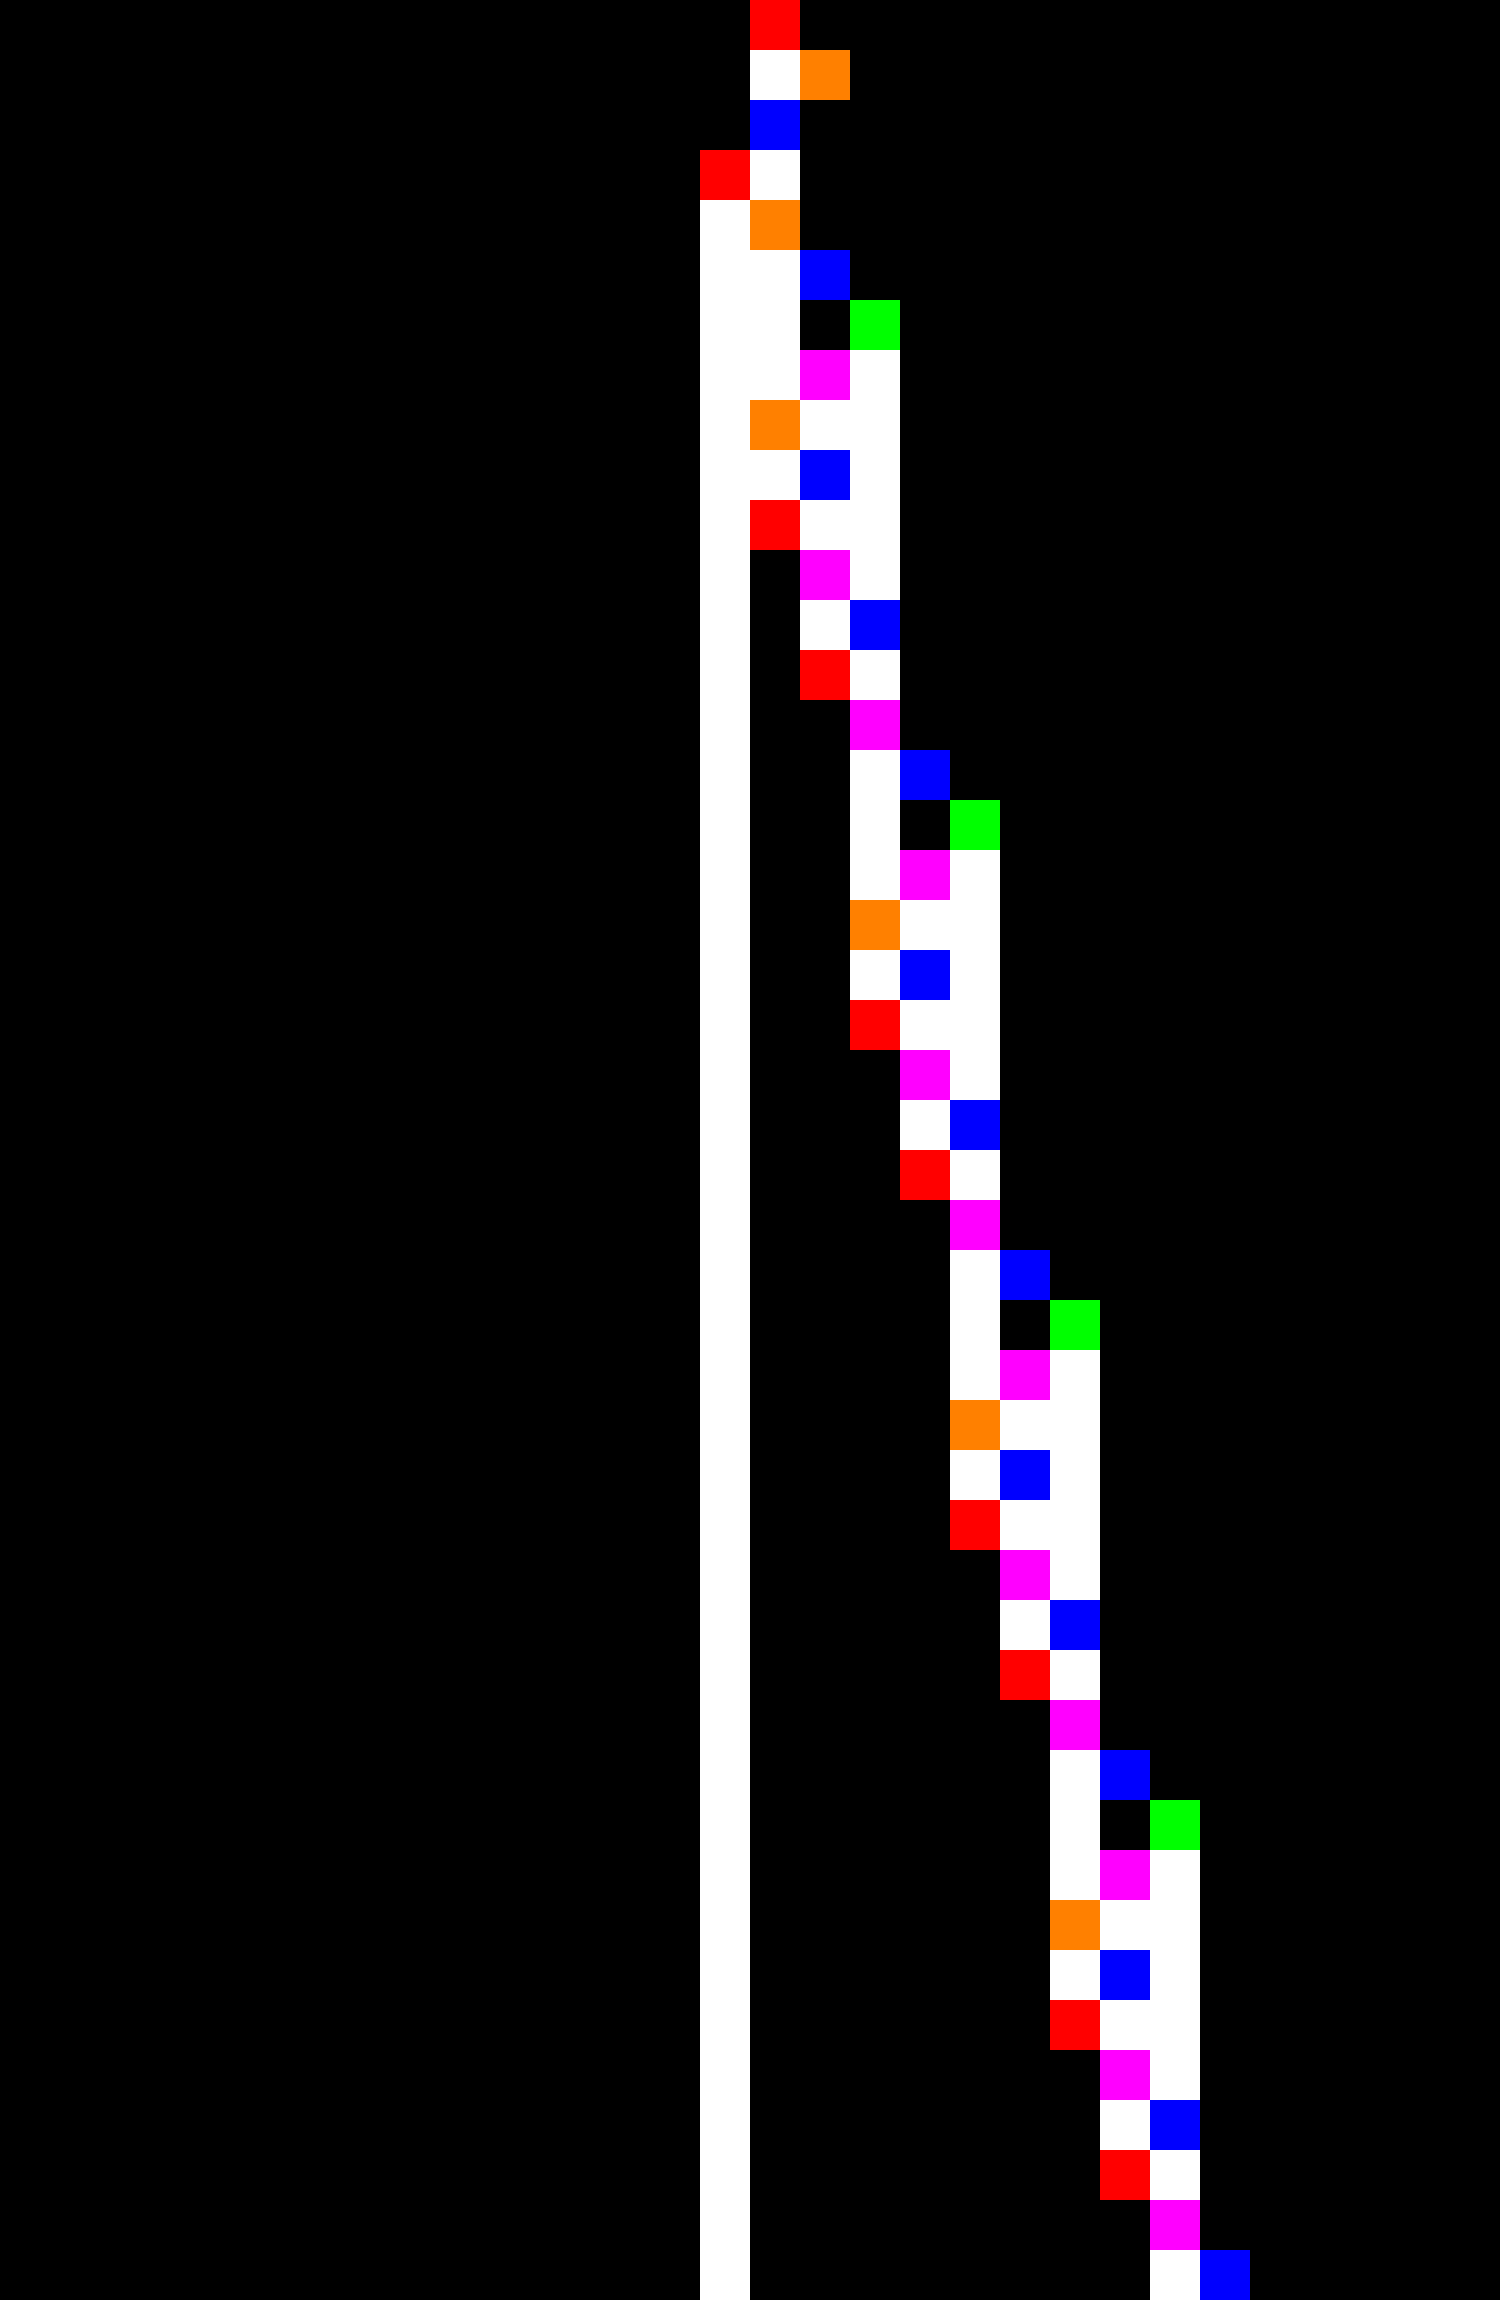
\includegraphics[width=0.5\textwidth]{figures/space-time-diagrams/translated_cycler_44394115.pdf}
    % \hspace{2ex}
    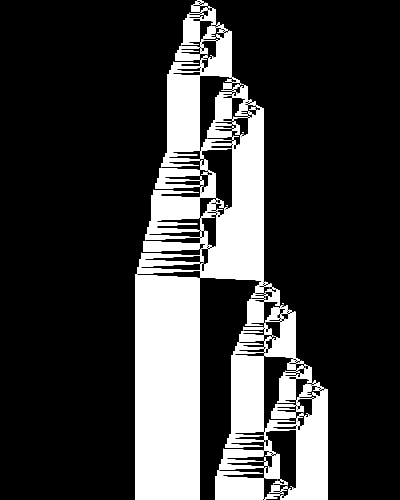
\includegraphics[width=0.5\textwidth]{figures/space-time-diagrams/ngramcps_LRU_35409542.png}

    \caption{10,000-step space-time diagram of a ``fractal-looking'' 5-state Turing machines that is solved by the LRU augmentation but has no known solution with standard \ngramcps or the fixed-length history augmentation, see Section~\ref{sec:n-gramCPS:augmentations}. See \url{https://bbchallenge.org/1RB0RA_1LC---_1RC1LD_0LE1RA_0LC0LE}.}\label{fig:ngram-cps-more}
\end{figure}




\newcommand{\leftngram}{left\xspace}
\newcommand{\rightngram}{right\xspace}
\newcommand{\middlesymbol}{middle\xspace}

\begin{algorithm}
    \caption{{\sc decider-NGramCPS}}\label{alg:NGramCPS}

    \begin{algorithmic}[1]
        \State{\textbf{Input:} A Turing machine $\mathcal{M}$, the zero symbol of the alphabet $\alphabet_0$, the size of the n-grams $n > 0$.}
        \State{\textbf{Output:} \NONHALT if the decider detects that the machine doesn't halt and `UNKNOWN' otherwise.}

        \State $g_0 = (\alphabet_0)^n$ \Comment{The zero n-gram consists of $n$ zero symbols}
        \State $L = \{ g_0 \}$ \Comment{The seen left n-grams}
        \State $R = \{ g_0 \}$ \Comment{The seen right n-grams}
        \State $C =$ \{\{.\leftngram $=$ $g_0$, .\rightngram $=$ $g_0$, .state $=$ \stateA, .\middlesymbol $=$ $\alphabet_0$ \}\} \Comment{The seen local configurations}
        \While{true}\label{alg:NGramCPS:line:whileTrue}
        \State $V = C$
        \State any\_updates $=$ false
        \While{$|V| \neq 0$}
        \State $c = V.\textbf{pop}()$
        \State $c' = c$
        \State $\{w,d,s\}$ $=$ $\mathcal{M}$(c.state, c.\middlesymbol) \Comment{Transition's write symbol, move direction, and next state}
        \State \If{$s$ is undefined} \Comment{Undefined transition is met, we cannot conclude}
        \State \textbf{return} UNKNOWN\label{alg:NGramCPS:line:unknown}
        \EndIf
        \State \If{$d$ is Right}
        \State Add $c.\text{\leftngram}$ to $L$ \label{alg:NGramCPS:line:insertL}
        \State Set $c'.\text{\leftngram}$ to the last $r-1$ symbols of $c.\text{\leftngram}$ followed by $w$
        \State Set $c'.\text{\middlesymbol}$ to the first symbol of $c.\text{\rightngram}$
        \For{each ngram $r\in R$ starting with the last $r-1$ symbols of $c.\text{\rightngram}$}
        \State Set $c'.\text{\rightngram}$ to $r$
        \If{$c'$ is not in $C$}
        \State \tabi Insert $c'$ in $C$ \label{alg:NGramCPS:line:insertInConfSet}
        \State \tabi Insert $c'$ in $V$ \label{alg:NGramCPS:line:insertInConfSetToVisit}
        \State \tabi any\_updates $=$ true
        \EndIf
        \EndFor
        \EndIf
        \State \If{$d$ is Left} \label{alg:NGramCPS:line:moveLeft}
        \State Add $c.\text{\rightngram}$ to $R$
        \State Set $c'.\text{\rightngram}$ to the first $r-1$ symbols of $c.\text{\rightngram}$ preceded by $w$
        \State Set $c'.\text{\middlesymbol}$ to the last symbol of $c.\text{\leftngram}$
        \For{each ngram $l \in L$ ending with the first $r-1$ symbols of $c.\text{\leftngram}$}
        \State Set $c'.\text{\leftngram}$ to $l$
        \If{$c'$ is not in $C$}
        \State \tabi Insert $c'$ in $C$
        \State \tabi Insert $c'$ in $V$
        \State \tabi any\_updates $=$ true
        \EndIf
        \EndFor
        \EndIf
        \EndWhile
        \State \If{\textbf{not} any\_updates}
        \State \textbf{return} \NONHALT\label{alg:NGramCPS:line:nonhalt} \Comment{Set $C$ is closed, and does not include undefined transitions:\\ \tabi \tabi \tabi \tabi \tabi \tabi \tabi \tabi \tabi \tabi \tabi \space \space \space \space the machine doesn't halt}
        \EndIf

        \EndWhile
    \end{algorithmic}
\end{algorithm}
